\documentclass[12pt,a4paper]{extarticle}
\usepackage[utf8]{inputenc}
\usepackage[T5]{fontenc}
\usepackage{geometry}
\geometry{a4paper, left=1.5cm, right=1cm, top=1.5cm, bottom=1.5cm, headheight=20pt, headsep=15pt, footskip=28pt}
\usepackage{enumitem}
\usepackage{amssymb}
\usepackage{tikz}
\usetikzlibrary{patterns, patterns.meta} % Thêm patterns.meta vào đây
% Gọi package nằm trong thư mục con template
\usepackage{../template/mngocbox}

\begin{document}

% Sử dụng ngoặc vuông [...] để thay đổi linh hoạt các thông số
\makeheadbox[headerright={Tổng ôn 10-11},chude={CHỦ ĐỀ 07},tieude={Dãy số},dinhdang={Đại số},lop={12 },gv={Nguyễn Lê Minh Ngọc}]

\vspace{2em}
\makeheading{I}{Tóm tắt lý thuyết}
\noindent\textbf{A. DÃY SỐ}

\noindent\textbf{1. Định nghĩa}
\vspace{0.2cm}
\noindent\textit{Dãy số vô hạn.}
\begin{itemize}
    \item Mỗi hàm số $u$ xác định trên tập các số nguyên dương $\mathbb{N}^*$ được gọi là một dãy số vô hạn (gọi tắt là dãy số), kí hiệu là $u = u(n)$.
    \item Ta thường viết $u_n$ thay cho $u(n)$ và kí hiệu dãy số $u = u(n)$ bởi $(u_n)$, do đó dãy số $(u_n)$ được viết dưới dạng khai triển $u_1, u_2, u_3, \dots, u_n, \dots$ Số $u_1$ gọi là số hạng đầu, $u_n$ là số hạng thứ $n$ và gọi là số hạng tổng quát của dãy số.
\end{itemize}
\noindent\textbf{Chú ý:} Nếu $\forall n \in \mathbb{N}^*$, $u_n = c$ thì $(u_n)$ được gọi là dãy số không đổi.
\vspace{0.4cm}

\vspace{0.4cm}
\noindent\textit{Dãy số hữu hạn.}
\begin{itemize}
    \item Mỗi hàm số $u$ xác định trên tập $M = \{1; 2; 3; \dots, m\}$ với $m \in \mathbb{N}^*$ được gọi là một dãy số hữu hạn.
    \item Dạng khai triển của dãy số hữu hạn là $u_1, u_2, \dots, u_m$. Số $u_1$ gọi là số hạng đầu, số $u_m$ gọi là số hạng cuối.
\end{itemize}
\vspace{0.4cm}

\noindent\textbf{2. Cách cho một dãy số}

\noindent Một dãy số có thể cho bằng:
\begin{itemize}
    \item Liệt kê các số hạng (chỉ dùng cho các dãy hữu hạn và có ít số hạng);
    \item Công thức của số hạng tổng quát;
    \item Phương pháp mô tả;
    \item Phương pháp truy hồi.
\end{itemize}

\vspace{0.3cm}
\noindent\textbf{Chú ý:}
\begin{itemize}
    \item Dãy số gồm tất cả các số nguyên tố ở Ví dụ được cho bởi phương pháp mô tả (số hạng thứ $n$ là số nguyên tố thứ $n$). Cho đến nay người ta vẫn chưa biết có hay không một công thức tính số nguyên tố thứ $n$ theo $n$ (với $n$ bất kì), hoặc là một hệ thức tính số nguyên tố thứ $n$ theo một vài số nguyên tố đứng trước nó.
    \item Để có hình ảnh trực quan về dãy số, ta thường biểu diễn các số hạng của nó trên trục số.
    
    Chẳng hạn, xét dãy số $(u_n)$ với $u_n = \dfrac{(-1)^n}{2^n}$. Năm số hạng đầu của dãy số này là $u_1 = -\dfrac{1}{2}$, $u_2 = \dfrac{1}{4}$, $u_3 = -\dfrac{1}{8}$, $u_4 = \dfrac{1}{16}$, $u_5 = -\dfrac{1}{32}$ và được biểu diễn trên trục số.
\end{itemize}
\vspace{0.4cm}

\noindent\textbf{3. Dãy số tăng, dãy số giảm}
\begin{itemize}
    \item Dãy số $(u_n)$ được gọi là dãy số tăng nếu $u_{n+1} > u_n$ với mọi $n \in \mathbb{N}^*$.
    \item Dãy số $(u_n)$ được gọi là dãy số giảm nếu $u_{n+1} < u_n$ với mọi $n \in \mathbb{N}^*$.
\end{itemize}
\noindent\textbf{Chú ý:} Không phải mọi dãy số đều là dãy số tăng hay dãy số giảm. Chẳng hạn, dãy số $(u_n)$ với $u_n = (-1)^n$ có dạng khai triển: $-1; 1; -1; 1; -1; \dots$ không là dãy số tăng, cũng không là dãy số giảm.
\vspace{0.3cm}

\vspace{0.4cm}
\noindent\textbf{4. Dãy số bị chặn}
\begin{itemize}
    \item Dãy số $(u_n)$ được gọi là bị chặn trên nếu tồn tại một số $M$ sao cho $u_n \le M$ với mọi $n \in \mathbb{N}^*$.
    \item Dãy số $(u_n)$ được gọi là bị chặn dưới nếu tồn tại một số $m$ sao cho $u_n \ge m$ với mọi $n \in \mathbb{N}^*$.
    \item Dãy số $(u_n)$ được gọi là bị chặn nếu nó vừa bị chặn trên, vừa bị chặn dưới; tức là tồn tại các số $m$ và $M$ sao cho $m \le u_n \le M$ với mọi $n \in \mathbb{N}^*$.
\end{itemize}
\vspace{0.3cm}

\noindent\textbf{B. CẤP SỐ CỘNG}

\noindent\textbf{1. Định nghĩa}
\begin{itemize}
    \item Cấp số cộng là một dãy số (hữu hạn hay vô hạn), trong đó kể từ số hạng thứ hai, mỗi số hạng đều bằng số hạng đứng ngay trước nó cộng với một số không đổi $d$. Số $d$ được gọi là công sai của cấp số cộng.
    \item Cấp số cộng $(u_n)$ với công sai $d$ được cho bởi hệ thức truy hồi
    \[ u_n = u_{n-1} + d \text{ với } n \ge 2. \]
\end{itemize}

\vspace{0.4cm}
\noindent\textbf{2. Số hạng tổng quát}
\noindent Nếu cấp số cộng $(u_n)$ có số hạng đầu $u_1$ và công sai $d$ thì số hạng tổng quát $u_n$ được xác định bởi công thức:
\[ u_n = u_1 + (n - 1)d \text{ với } n \ge 2. \]

\vspace{0.4cm}
\noindent\textbf{3. Tổng $n$ số hạng đầu của một cấp số cộng}
\noindent Cho cấp số cộng $(u_n)$ với công sai $d$. Đặt $S_n = u_1 + u_2 + \dots + u_n$. Khi đó
\[ S_n = \frac{n}{2}[2u_1 + (n - 1)d]. \]
\noindent\textbf{Chú ý:} Sử dụng công thức $u_n = u_1 + (n - 1)d$, ta có thể viết tổng $S_n$ dưới dạng
\[ S_n = \frac{n(u_1 + u_n)}{2}. \]

\vspace{0.6cm}
\noindent\textbf{C. CẤP SỐ NHÂN}

\noindent\textbf{1. Định nghĩa}
\begin{itemize}
    \item Cấp số nhân là một dãy số (hữu hạn hay vô hạn), trong đó kể từ số hạng thứ hai, mỗi số hạng đều là tích của số hạng đứng ngay trước nó với một số không đổi $q$. Số $q$ được gọi là công bội của cấp số nhân.
    \item Cấp số nhân $(u_n)$ với công bội $q$ được cho bởi hệ thức truy hồi
    \[ u_n = u_{n-1} \cdot q \text{ với } n \ge 2. \]
\end{itemize}

\vspace{0.4cm}
\noindent\textbf{2. Số hạng tổng quát}
\begin{itemize}
    \item Nếu cấp số nhân $(u_n)$ có số hạng đầu $u_1$ và công bội $q$ thì số hạng tổng quát $u_n$ được xác định bởi công thức:
    \[ u_n = u_1 \cdot q^{n-1} \text{ với } n \ge 2. \]
\end{itemize}

\noindent\textbf{3. Tổng $n$ số hạng đầu của một cấp số nhân}
\begin{itemize}
    \item Cho cấp số nhân $(u_n)$ với công bội $q \ne 1$. Đặt $S_n = u_1 + u_2 + u_3 + \dots + u_n$. Khi đó:
    \[ S_n = \frac{u_1(1 - q^n)}{1 - q}. \]
\end{itemize}

\makeheading{II}{Bài tập tự luyện}
\noindent\textbf{1.} Cho dãy số $(u_n)$, biết $u_n = \dfrac{2n - 1}{n + 2}$ ($n \in \mathbb{N}^*$). Hỏi $\dfrac{19}{10}$ là số hạng thứ bao nhiêu của dãy số?

\noindent\textbf{2.} Với mỗi số nguyên dương $n$, lấy $n + 6$ điểm cách đều nhau trên đường tròn. Nối mỗi điểm với điểm cách nó hai điểm trên đường tròn đó để tạo thành các ngôi sao như hình vẽ. Gọi $u_n$ là số đo góc ở đỉnh tính theo đơn vị độ của mỗi ngôi sao thì ta được dãy số $(u_n)$. Tìm công thức của số hạng tổng quát $u_n$.
\begin{center}
    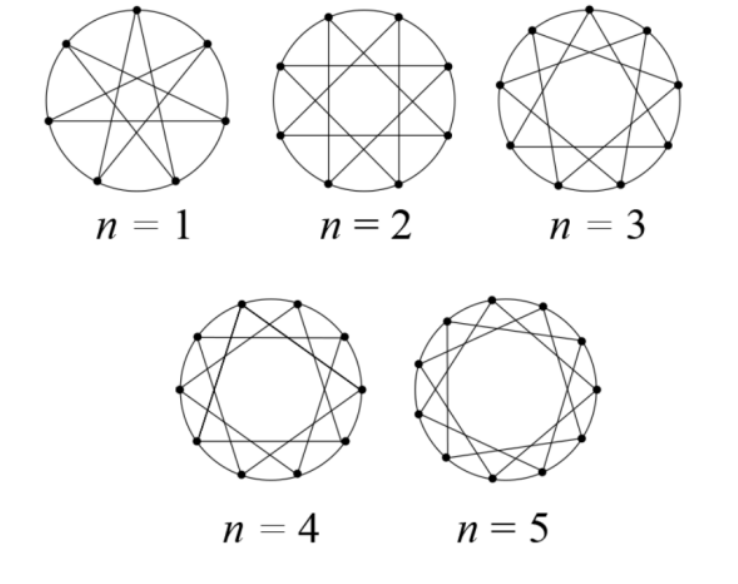
\includegraphics[width=0.5\textwidth]{14.3.png}
\end{center}

\noindent\textbf{3.} Một công ty dược phẩm đang thử nghiệm một loại thuốc mới. Một thí nghiệm bắt đầu với $1{,}0 \times 10^9$ vi khuẩn. Một liều thuốc được sử dụng sau mỗi bốn giờ có thể tiêu diệt $4{,}0 \times 10^8$ vi khuẩn. Giữa các liều thuốc, số lượng vi khuẩn tăng lên 25\%. Tìm số vi khuẩn còn sống trước lần sử dụng thuốc thứ năm.

\noindent\textbf{4.} Chiều cao (đơn vị: centimét) của một đứa trẻ $n$ tuổi phát triển bình thường (Nguồn: \textit{https://bibabo.vn}) được cho bởi công thức:
\[ x_n = 75 + 5(n - 1) \]
\noindent a) Một đứa trẻ phát triển bình thường có chiều cao năm 3 tuổi là bao nhiêu centimét?\\
\noindent b) Dãy số $(x_n)$ có là một cấp số cộng không? Trung bình một năm, chiều cao mỗi đứa trẻ phát triển bình thường tăng lên bao nhiêu centimét?

\noindent\textbf{5.} Chuông đồng hồ ở một toà tháp đánh số tiếng đúng bằng số giờ và cứ mỗi 30 phút không phải là giờ đúng thì đánh 1 tiếng chuông. Hỏi bắt đầu từ lúc 1 giờ đêm đến 12 giờ trưa, chuông đồng hồ đó đã đánh tất cả bao nhiêu tiếng?

\noindent\textbf{6.} Anh Dũng kí hợp đồng lao động trong 10 năm với phương án trả lương như sau: Năm thứ nhất, tiền lương của anh Dũng là 120 triệu đồng. Kể từ năm thứ hai trở đi, mỗi năm tiền lương của anh Dũng được tăng lên 10\%. Tính tổng số tiền lương anh Dũng lĩnh được trong 10 năm đầu đi làm (làm tròn kết quả đến hàng đơn vị theo đơn vị triệu đồng).
\vspace{0.6cm}

\noindent\textbf{7.} Một tháp 10 tầng có diện tích sàn của tầng dưới cùng là $6144\text{ m}^2$. Tính diện tích mặt sàn tầng trên cùng, biết rằng diện tích mặt sàn mỗi tầng bằng nửa diện tích mặt sàn tầng ngay bên dưới.
\vspace{0.6cm}
\begin{center}
    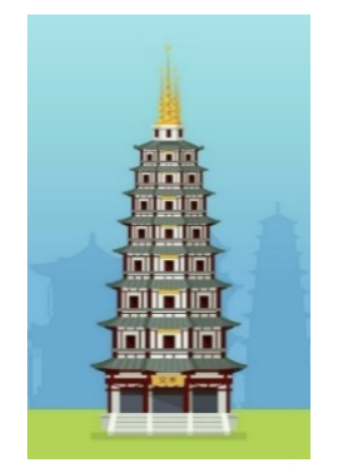
\includegraphics[width=0.3\textwidth]{14.13.png}
\end{center}

\noindent\textbf{8.} Để tích luỹ tiền cho việc học đại học của con gái, cô Hoa quyết định hằng tháng bỏ ra 500 nghìn đồng vào tài khoản tiết kiệm, được trả lãi 0,5\% cộng dồn hằng tháng. Cô bắt đầu chương trình tích luỹ này khi con gái cô tròn 3 tuổi. Cô ấy sẽ tích luỹ được bao nhiêu tiền vào thời điểm gửi khoản tiền thứ 180? Lúc này con gái cô Hoa bao nhiêu tuổi?

\makeheading{III}{Bài tập làm thêm}

\noindent\textbf{1.} Giá của một chiếc máy photocopy lúc mới mua là 50 triệu đồng. Biết rằng giá trị của nó sau mỗi năm sử dụng chỉ còn 75\% giá trị trong năm liền trước đó. Tính giá trị còn lại của chiếc máy photocopy đó sau mỗi năm, trong khoảng thời gian 5 năm kể từ khi mua.

\noindent\textbf{2.} Bác An gửi tiết kiệm 200 triệu đồng kì hạn 3 tháng, với lãi suất 3\% một năm. Số tiền (triệu đồng) cả vốn lẫn lãi mà bác An nhận được sau $n$ quý (mỗi quý là 3 tháng) sẽ là:
\[ A_n = 200\left(1 + \frac{0{,}03}{4}\right)^n, \quad n = 0, 1, 2, \dots \]
\noindent Tìm số tiền bác An nhận được sau 2 năm.

\noindent\textbf{3.} Cho dãy số $(u_n)$ biết $u_1 = -2$, $u_{n+1} = \dfrac{u_n}{1 - u_n}$ với $n \in \mathbb{N}^*$. Đặt $v_n = \dfrac{u_n + 1}{u_n}$ với $n \in \mathbb{N}^*$.\\
\noindent a) Chứng minh rằng dãy số $(v_n)$ là một cấp số cộng. Tìm số hạng đầu, công sai của cấp số cộng đó.\\
\noindent b) Tìm công thức của $v_n, u_n$ tính theo $n$.\\
\noindent c) Tính tổng $S = \dfrac{1}{u_1} + \dfrac{1}{u_2} + \dfrac{1}{u_3} + \dots + \dfrac{1}{u_{20}}$.

\noindent\textbf{4.} Các khúc gỗ được xếp như Hình 2. Lượt thứ nhất có 21 khúc, lượt thứ hai có 20 khúc, ..., lượt trên cùng có 15 khúc. Tính tổng số khúc gỗ đã được xếp.
\begin{center}
    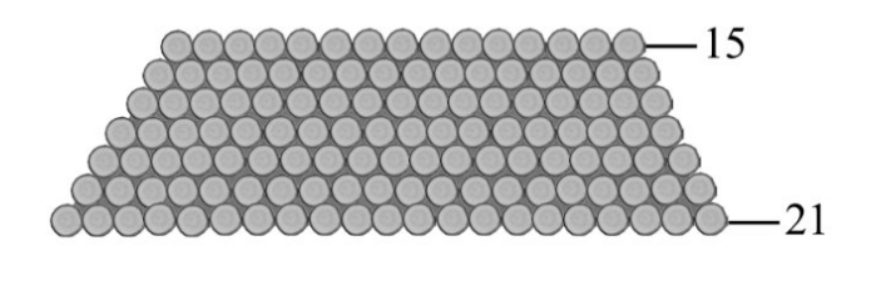
\includegraphics[width=0.5\textwidth]{14.8.png}
\end{center}

\noindent\textbf{5.} Một bức tường trang trí có dạng hình thang, rộng $2{,}4\text{ m}$ ở đáy và rộng $1{,}2\text{ m}$ ở đỉnh (hình vẽ bên). Các viên gạch hình vuông có kích thước $10\text{ cm} \times 10\text{ cm}$ phải được đặt sao cho mỗi hàng ở phía trên chứa ít hơn một viên so với hàng ở ngay phía dưới nó.
\begin{center}
    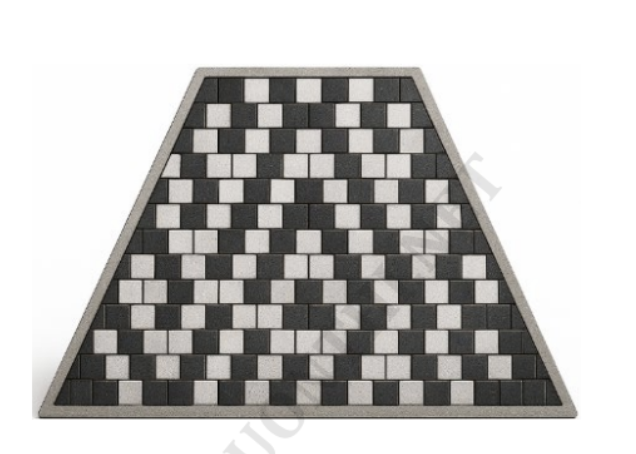
\includegraphics[width=0.5\textwidth]{14.9.png}
\end{center}

\noindent\textbf{6.} Một công ty mua một chiếc máy với giá 1 tỉ 200 triệu đồng. Công ty nhận thấy, trong vòng 5 năm đầu, tốc độ khấu hao là 25\%/ năm (tức là sau mỗi một năm, giá trị còn lại của chiếc máy bằng 75\% giá trị của năm trước đó).
\noindent a) Viết công thức tính giá trị của chiếc máy đó sau 1 năm, 2 năm.
\noindent b) Sau 5 năm, giá trị của chiếc máy đó còn khoảng bao nhiêu triệu đồng (làm tròn kết quả đến hàng đơn vị)?
\vspace{0.5cm}

\noindent\textbf{7.} Một khay nước có nhiệt độ $20^\circ\text{C}$ được đặt vào ngăn đá của tủ lạnh. Cho biết sau mỗi giờ, nhiệt độ của nước giảm đi 25\%. Tính nhiệt độ khay nước đó sau 4 giờ.
\begin{center}
    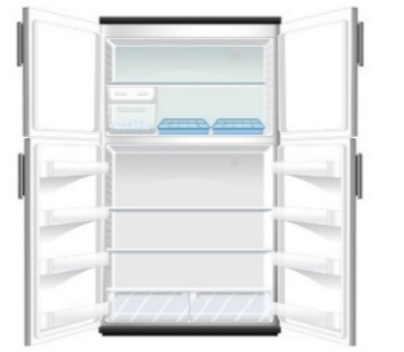
\includegraphics[width=0.3\textwidth]{14.14.png}
\end{center}
\end{document}